\documentclass{article}
\usepackage{ctex}
\usepackage{diagbox} % 加载宏包
\usepackage{geometry}
\usepackage{booktabs}
\usepackage{graphicx}
\usepackage[section]{placeins}
\geometry{a4paper,left=2.5cm,right=2cm,top=2.5cm,bottom=2cm}
\usepackage{float}
\usepackage{enumerate}
% 编写矩阵
\usepackage{amsmath,amssymb,amsfonts}
% 代码的编写
\usepackage{caption}
\usepackage[dvipsnames]{xcolor}  % 更全的色系
\usepackage{listings}  % 排代码用的宏包
\lstset{
    % framexleftmargin=2em
    xleftmargin=2em,xrightmargin=2em, aboveskip=1em,
    backgroundcolor = \color{yellow!10},    % 背景色:淡黄
    basicstyle = \small\ttfamily,           % 基本样式 + 小号字体
    % rulesepcolor= \color{ red!20!green!20!blue!20} ,
    rulesepcolor= \color{gray},             % 代码块边框颜色
    breaklines = true,                  % 代码过长则换行
    numbers = left,                     % 行号在左侧显示
    numberstyle = \small,               % 行号字体
    keywordstyle = \color{blue},            % 关键字颜色
    commentstyle =\color{green!100},        % 注释颜色
    stringstyle = \color{red!100},          % 字符串颜色
    frame = shadowbox,                  % 用(带影子效果)方框框住代码块
    showspaces = false,                 % 不显示空格
    columns = fixed,                    % 字间距固定
    escapeinside={(:}{:)},
    % escapeinside=``, % 英文分号中可写入中文
    % escapeinside={<@}{@>}              % 特殊自定分隔符:<@可以自己加颜色@>
    morekeywords = {as},                % 自加新的关键字(必须前后都是空格)
    deletendkeywords = {compile}        % 删除内定关键字;删除错误标记的关键字用deletekeywords删!
}
\title{液体粘滞系数测量实验}
\author{姓名:卢杨 \quad 学号:PB23000043}
\begin{document}
\maketitle
\section{实验数据}

\begin{table}[!hbtp]
    \begin{center}
    \caption{小球数据}
    \begin{tabular}{l|c|c|c|c|c|r}
        % \textbf{磁针距离$l/(10^{-2})m$} & 19 & 21 & 23 & 25 & 27 & 29 \\
        % $\ln l$ & -1.660731 & -1.560648 & -1.469676 & -1.386294 & -1.309333 & -1.237874 \\
        \hline
        大球$r(/10^{-2}m)$ & 0.3018 & 0.3020 & 0.3020 & 0.3015 & 0.3021 & 0.3018 \\
        大球$m(/10^{-3}kg)$ & 0.1136 & 0.1136 & 0.1136 & 0.1137 & 0.1128 & 0.1134 \\
        大球$t(/s)$ & 4.16 & 4.23 & 4.21 & 4.17 & 4.20 & 4.23 \\
        中球$r(/10^{-2}m)$ & 0.2518 & 0.2520 & 0.2516 & 0.2518 & 0.2517 & 0.2517 \\
        中球$m(/10^{-3}kg)$ & 0.0657 & 0.0656 & 0.0655 & 0.0655 & 0.0651 & 0.0653 \\
        中球$t(/s)$ & 5.87 & 6.03 & 5.96 & 5.94 & 5.88 & 6.00 \\
        小球$r(/10^{-2}m)$ & 0.1820 & 0.1820 & 0.1820 & 0.1821 & 0.1820 & 0.1819 \\
        小球$m(/10^{-3}kg)$ & 0.0245 & 0.0243 & 0.0245 & 0.0248 & 0.0246 & 0.0246 \\
        小球$t(/s)$ & 11.05 & 10.97 & 11.29 & 11.11 & 11.22 & 11.20 \\
    \end{tabular}
    \end{center}
\end{table}


\begin{table}[!hbtp]
    \begin{center}
    \caption{客观数据}
    \begin{tabular}{l|c|c|r}
        \hline
        密度$\rho _0/10^{3}kg/m^3$ &0.956 & 0.956 & 0.956 \\
        温度$T$ & 25.1 & 25.1 & 25.1 \\
        桶直径$D/10^{-2}m$ & 8.160 & 8.154 & 8.162 \\
        桶高度$h/10^{-2}m$ & 42.1 & 42.2 & 42.2 \\
        匀速区间$l/10^{-2}m$ & 18.75 \\
    \end{tabular}
    \end{center}
\end{table}

\section{实验数据处理}

\subsection{求平均值}

\begin{table}[!hbtp]
    \begin{center}
    \caption{球的数据平均值}
    \begin{tabular}{l|r}

        \hline
        大球$r(/10^{-2}m)$ & 0.3018 \\
        大球$m(/10^{-3}kg)$ & 0.1135 \\
        大球$t(/s)$ & 4.2 \\
        中球$r(/10^{-2}m)$ & 0.2517 \\
        中球$m(/10^{-3}kg)$ & 0.06545 \\
        中球$t(/s)$ & 5.9467 \\
        小球$r(/10^{-2}m)$ & 0.1820 \\
        小球$m(/10^{-3}kg)$ & 0.02455 \\
        小球$t(/s)$ & 11.14 \\

    \end{tabular}
    \end{center}
\end{table}

\begin{table}[!hbtp]
    \begin{center}
    \caption{客观数据平均值}
    \begin{tabular}{l|r}

        \hline
        密度$\rho _0/10^{3}kg/m^3$ &0.956 \\
        温度$T$ & 25.1 \\
        桶直径$D/10^{-2}m$ & 8.1587 \\
        桶高度$h/10^{-2}m$ & 42.167 \\

    \end{tabular}
    \end{center}
\end{table}

\newpage

\subsection{求平均速度}

使用公式$v=\frac{l}{t}$即可计算求得

\begin{table}[!hbtp]
    \begin{center}
    \caption{球的速度平均值}
    \begin{tabular}{l|r}

        \hline
        大球$v(/m\cdot s^{-1})$ & 0.04464 \\
        中球$v(/m\cdot s^{-1})$ & 0.03153 \\
        小球$v(/m\cdot s^{-1})$ & 0.01683 \\

    \end{tabular}
    \end{center}
\end{table}

\subsection{粘滞系数粗略计算}

使用公式进行计算
$$
\eta =\frac{(m-\rho _0V)g}{6\pi vr}
$$

其中,取$g=9.8m/s^{2}$,有

\begin{table}[!hbtp]
    \begin{center}
    \caption{粘滞系数粗略计算}
    \begin{tabular}{l|r}

        \hline
        大球 & 0.012723953962248125 \\
        中球 & 0.010112643568152217 \\
        小球 & 0.006936515802236658 \\

    \end{tabular}
    \end{center}
\end{table}




\subsection{粘滞系数修正}

我们对雷诺数进行计算
$$R_e=\frac{2rv\rho _0}{\eta }$$

得到的

\begin{table}[!hbtp]
    \begin{center}
    \caption{雷诺数}
    \begin{tabular}{l|r}

        \hline
        大球 & 20.250368923783547 \\
        中球 & 15.008907960039814 \\
        小球 & 8.44372299050132 \\

    \end{tabular}
    \end{center}
\end{table}

通过一级、二级、三级公式修正的结果如下

\begin{table}[!hbtp]
    \begin{center}
    \caption{粘滞系数修正}
    \begin{tabular}{l|r}
        \hline
        大球$\eta _0$ & 0.010555639571414683 \\
        大球$\eta _1$ & -0.03775650328572819 \\
        大球$\eta _2$ & -0.05792156705830437 \\
        中球$\eta _0$ & 0.00863779055194359 \\
        中球$\eta _1$ & -0.019820910050634896 \\
        中球$\eta _2$ & -0.032349243540126166 \\
        小球$\eta _0$ & 0.0061776257546557189 \\
        小球$\eta _1$ & -0.00480425261159204 \\
        小球$\eta _2$ & -0.01053358787947256 \\

    \end{tabular}
    \end{center}
\end{table}




\subsection{结果分析和讨论}

我们可以看到,其实到第二级修正之后就开始不符合实际了,其实这是因为雷诺数$R_e$的值过大

采用原始式子

$$
\eta =\frac{1}{18}\frac{(\rho _0-\rho )gd^2}{v(1+1.24\frac{d}{2R})(1+3.3\frac{d}{2h})(1+\frac{3}{16}R_e)}
$$

可以进行重新计算,得到以下结果


\begin{table}[!hbtp]
    \begin{center}
    \caption{粘滞系数修正}
    \begin{tabular}{l|r}
        \hline
        大球$\eta $ & 0.0022004924781837496 \\
        中球$\eta $ & 0.0022646578424000913 \\
        小球$\eta $ & 0.002391464227460848 \\
    \end{tabular}
    \end{center}
\end{table}

可以看到这样修正之后的结果符合实际



% \subsection{实验仪器}
% 高灵敏度特斯拉计量程$0\sim 3000mT$,分辨率为$0.01mT$;亥姆霍兹线圈;
% 磁力摆$2$个;直流电源;质量相同的配重螺帽两个;米尺和秒表
% \subsection{实验方案设计}
% \subsubsection*{周期数的预测}
% 实验要求$T$的不确定度满足:$U_T\leq 0.5\%$,而用秒表测量时间的不确定度$\Delta t$约为$0.2s$。
% 假设测量的周期数是$n$次,那么$$U_T=\frac{\Delta t}{nT}$$

% 其中$T$为周期,在$I=0.3A$时进行粗测,得到的$T\thickapprox 0.5s$,有$n\approx 80$,实际测量选择测量80次
% \subsubsection*{设计实验对转动惯量和磁矩进行测量}
% 在研究$I$与$B$之间的关系时,得到$(2)$式的$k$值,同时可以通过测量得到$I$与$T^{-2}$的关系,其中$B_0$是局域场
% \begin{equation}
%     B=B_0+kI=\frac{4 \pi^2J}{m}\frac{1}{T^2}
% \end{equation}
% \begin{equation}
%     I=\frac{4 \pi^2J}{km}\frac{1}{T^2}-\frac{B_0}{k}
% \end{equation}
% 那么
% \begin{equation}
%     I=a\frac{1}{T^2}+b \Longrightarrow \frac{J}{m}=\frac{ak}{4\pi ^2} \quad |B_0|=kb
% \end{equation}

% 在测量转动惯量时,通过增加一个转动惯量,可以改变$J$的值,再通过$(1)$式有$$T_1=2\pi \sqrt{\frac{J}{mB}} \quad T_2=2\pi \sqrt{\frac{J+\Delta J}{mB}}$$
% 将两个周期进行比较得到$$\frac{T_2}{T_1}=\sqrt{\frac{J+\Delta J}{J}} \Longrightarrow \frac{\Delta J}{J}=(\frac{T_2}{T_1})^2-1$$
% 最后得到
% \begin{equation}
%     J=\Delta J[(\frac{T_2}{T_1})^2-1]^{-1}
% \end{equation}
% 最后可以通过$(5)$式得到磁矩$m$的值
% \begin{equation}
%     m=\frac{4\pi ^2J}{ak}
% \end{equation}
% \subsection{实验内容}
% \begin{itemize}
%     \item 测量磁针处局域磁场水平分量的大小
%     \begin{itemize}
%         \item 测量磁场大小与电流之间的关系
%         \item 选取适当的测量范围,测量不同电流下磁针的振动周期。通过作图给出局域磁场水平分量的值
%     \end{itemize}
%     \item 测量磁针的磁矩以及转动惯量
%     \begin{itemize}
%         \item 设计实验方案,用于测量磁针的转动惯量以及磁针的磁矩
%         \item 测量磁针的转动惯量以及它的磁矩
%     \end{itemize}
%     \item 地磁场中耦合磁针运动的观察与测量(同相位耦合运动的圆频率为:$\omega$,反相位耦合运动的圆频率为:$\omega^*$,单独一个小磁针的圆频率为:$\omega_0$)
%     \begin{itemize}
%         \item 比较$\omega$、$\omega^*$、$\omega_0$三者的大小
%         \item 改变磁针之间的距离,测量三个圆频率随$L$的变化情况
%         \item 确定系数$\alpha $和$\beta$的值:(其中$\alpha$和$\beta$是常数,$M$是磁矩)
%         \begin{equation}
%             k'=\alpha\frac{M^2}{L^\beta}=\frac{1}{2}\left|\omega^2-\omega^{*2}\right|
%         \end{equation}
%     \end{itemize}
% \end{itemize}
% \section{实验结果与讨论}
% \subsection{探究亥姆霍兹线圈$B$与$I$的关系}

% \begin{figure}[H]
%     \centering
%     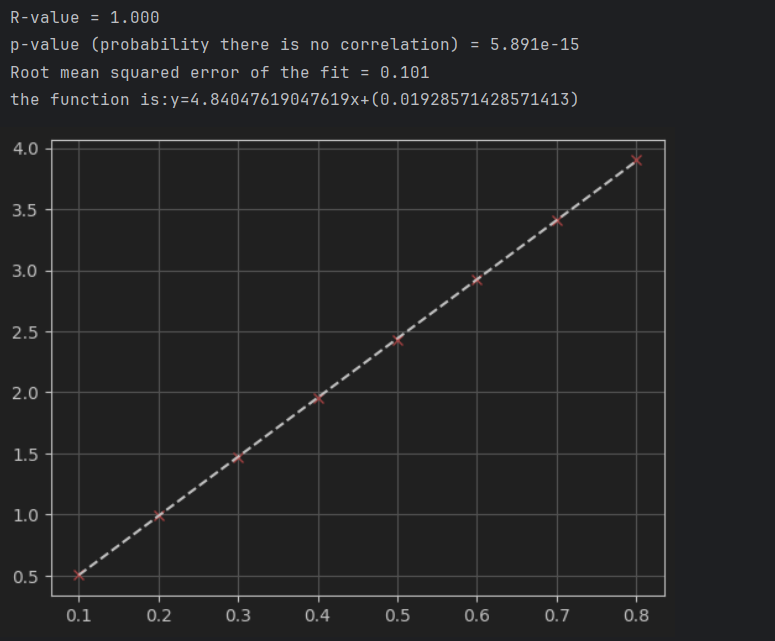
\includegraphics[width=12cm]{./img/B-T.png}
% \end{figure}

% \begin{table}[!hbtp]
%     \begin{center}
%     \caption{亥姆霍兹线圈$B$与$I$的关系}
%     \begin{tabular}{l|c|c|c|c|c|c|c|r}
%         \textbf{电流I(/A)} & \textbf{0.1} & \textbf{0.2} & \textbf{0.3} & \textbf{0.4} & \textbf{0.5} & \textbf{0.6} & \textbf{0.7} & \textbf{0.8} \\
%         \hline
%         磁场$B(/mT)$ & 0.51 & 0.99 & 1.47 & 1.95 & 2.43 & 2.92 & 3.41 & 3.90\\
%     \end{tabular}
%     \end{center}
% \end{table}

% 可以看到回归结果为$B=4.8405I+0.0193$,因此可以得到
% \begin{equation}
%     k=4.8405\times 10^{-3}T/A
% \end{equation}

% \subsection{$I$与周期$T^{-2}$求局域场分量$B_0$}
% 在实验中测量周期数是$n=80$次
% \begin{table}[!hbtp]
%     \begin{center}
%     \caption{$I$与周期$T^{-2}$的关系}
%     \begin{tabular}{l|c|c|r}
%         \textbf{电流I(/A)} & \textbf{总时长$nT(/s)$} & \textbf{周期$T(/s)$} & \textbf{$T^{-2}(/s^{-2})$} \\
%         \hline
%         0.01 & 99.11 & 1.238875 & 0.65154591 \\
%         \hline
%         0.015 & 68.79 & 0.859875 & 1.35247534 \\
%         \hline
%         0.02 & 56.23 & 0.702875 & 2.02415519 \\
%         \hline
%         0.025 & 49.67 & 0.620875 & 2.59412951 \\
%         \hline
%         0.03 & 43.41 & 0.542625 & 3.39625587 \\
%         \hline
%         0.035 & 39.36 & 0.492 & 4.13113887 \\
%     \end{tabular}
%     \end{center}
% \end{table}

% \begin{figure}[H]
%     \centering
%     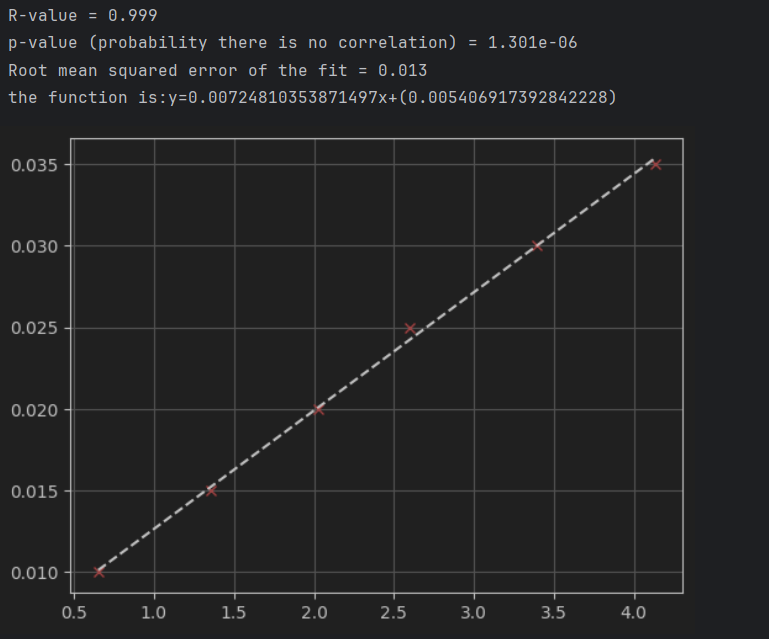
\includegraphics[width=12cm]{./img/T-2.png}
% \end{figure}

% 可以看到回归结果为$$I=7.248\times 10^{-3}\frac{1}{T^2}+5.407\times 10^{-3}$$

% 由$(5)$式和$(9)$式可以得到
% \begin{equation}
%     \frac{J}{m}=\frac{ak}{4\pi ^2}=\frac{7.248\times 10^{-3}\times 4.8405\times 10^{-3}}{4\times \pi^2}=8.887\times 10^{-7}
% \end{equation}
% \begin{equation}
%     \quad |B_0|=kb=4.8405\times 10^{-3}\times 5.407\times 10^{-3}=2.617\times 10^{-5}T=2.617 \times 10^{-2}mT
% \end{equation}

% 因此我们求得的局域场$B_0=2.617\times 10^{-2}mT$,
% 而回归结果中$b>0$可以知道测量时局域场$B_0$和亥姆霍兹线圈磁场方向相反

% \subsection{转动惯量和磁矩的测量}
% 在小磁针的两边加上两个螺帽,一个螺帽的质量为$m=0.72g$,螺帽距离小磁针中心的半径为$r=2.6cm$
% 那么转动惯量的增量为$\Delta J=2mr^2=9.7344\times 10^{-7}kg\cdot m^2$

% 我选取的是在$I=0.02A$时进行周期的再测量,测量的总时间结果为$nT_2=76.56s$

% 由$(6)$式可以得到转动惯量的值
% \begin{align*}
%     J&=\Delta J[(\frac{T_2}{T_1})^2-1]^{-1}=\Delta J[(\frac{nT_2}{nT_1})^2-1]^{-1} \\
%     &=9.7344\times 10^{-7}\times [(\frac{76.56}{56.23})^2-1]^{-1}=1.1401\times 10^{-6}kg\cdot m^2\\
% \end{align*}

% 通过$(7)$和$(10)$式可以得到磁矩的值
% $$m=\frac{4\pi ^2J}{ak}=\frac{1.1401\times 10^{-6}}{8.887\times 10^{-7}}=1.283A\cdot m^2$$
% \subsection{耦合小磁针的运动规律探究}
% \begin{table}[!hbtp]
%     \begin{center}
%     \caption{耦合小磁针的运动规律}
%     \begin{tabular}{l|c|c|c|c|c|r}
%         \textbf{磁针距离$l/(10^{-2})m$} & 19 & 21 & 23 & 25 & 27 & 29 \\
%         $\ln l$ & -1.660731 & -1.560648 & -1.469676 & -1.386294 & -1.309333 & -1.237874 \\
%         \hline
%         同相位$(nT/s)$ & 51.73 & 66.88 & 70.52 & 77.51 & 78.82 & 84.19 \\
%         $T/s$ & 0.646625 & 0.836 & 0.8815 & 0.968875 & 0.98525 & 1.052375 \\
%         $\omega/s^{-1}$ & 1.546491 & 1.196172 & 1.134430 & 1.032125 & 1.014971 & 0.950232 \\
%         \hline
%         反相位$(nT^*/s)$ & 72.93 & 79.32 & 84.27 & 86.22 & 88.39 & 90.60 \\
%         $T/s$ & 0.911625 & 0.9915 & 1.053375 & 1.07775 & 1.104875 & 1.1325 \\
%         $\omega^*/s^{-1}$ & 1.096942 & 1.008573 & 0.949330 & 0.927859 & 0.905080 & 0.883002 \\
%         \hline
%         $output$ & 0.594177 & 0.206804 & 0.192852 & 0.102180 & 0.105498 & 0.061624 \\
%         $\ln(output)$ & -0.520579 & -1.575982 & -1.645830 & -2.281022 & -2.249061 & -2.786710 \\
%     \end{tabular}
%     \end{center}
% \end{table}
% 没有耦合时的周期为$nT_0=101.44s$

% 可以很明显的看到随$L$的增大,周期明显增大,圆频率随$L$增大而减小

% 通过比较可以得到$$T<T^*<T_0\quad \omega >\omega ^*>\omega _0$$、

% 我将(8)式进行一些处理:
% \begin{equation}
%     \ln \alpha+2\ln M-\beta\ln L=ln(\frac{1}{2}\left|\omega^2-\omega^{*2}\right|)
% \end{equation}
% 将$output=\frac{1}{2}\left|\omega^2-\omega^{*2}\right|$作为一个整体进行考虑

% \begin{figure}[H]
%     \centering
%     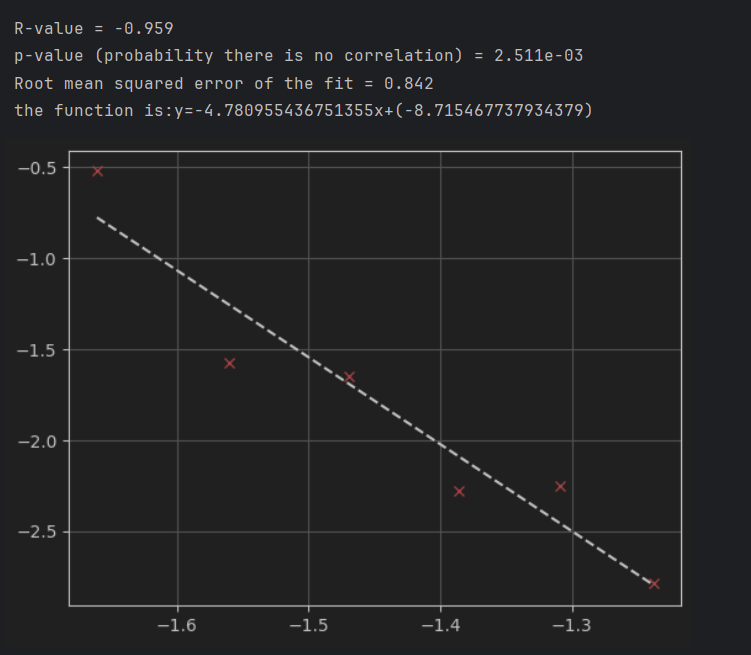
\includegraphics[width=12cm]{./img/a-b.png}
% \end{figure}

% 拟合结果为:$\ln(output)=-4.780955436751355\ln L-8.715467737934379$
% 有

% $$\begin{cases}
%     \beta=4.780955436751355 \\
%     \ln \alpha+2\ln M=-8.715467737934379
% \end{cases}$$

% 又由$M=1.283A\cdot m^2$可得

% $$\begin{cases}
%     \beta=4.781 \\
%     \alpha=9.965\times 10^{-5} \approx 1\times 10^{-5}
% \end{cases}$$

% \section{结论}
% 本文对亥姆霍兹线圈磁场与电流关系进行研究,进而对小磁针转动惯量、磁矩、局域磁场大小进行测量。
% 并且进一步对两个小磁针的耦合现象进行研究和讨论,发现同相位耦合的圆频率高于反相位耦合的圆频率,
% 但不管怎么样,圆频率在耦合状态下都是高于单一小磁针的圆频率的。测量结果表明,耦合系数$k'\propto L^{-\beta}(\beta \approx4.781)$

% \newpage
% \section*{附录:老师签字的实验数据照片}
% % \begin{figure}[H]
% %     \centering
% %     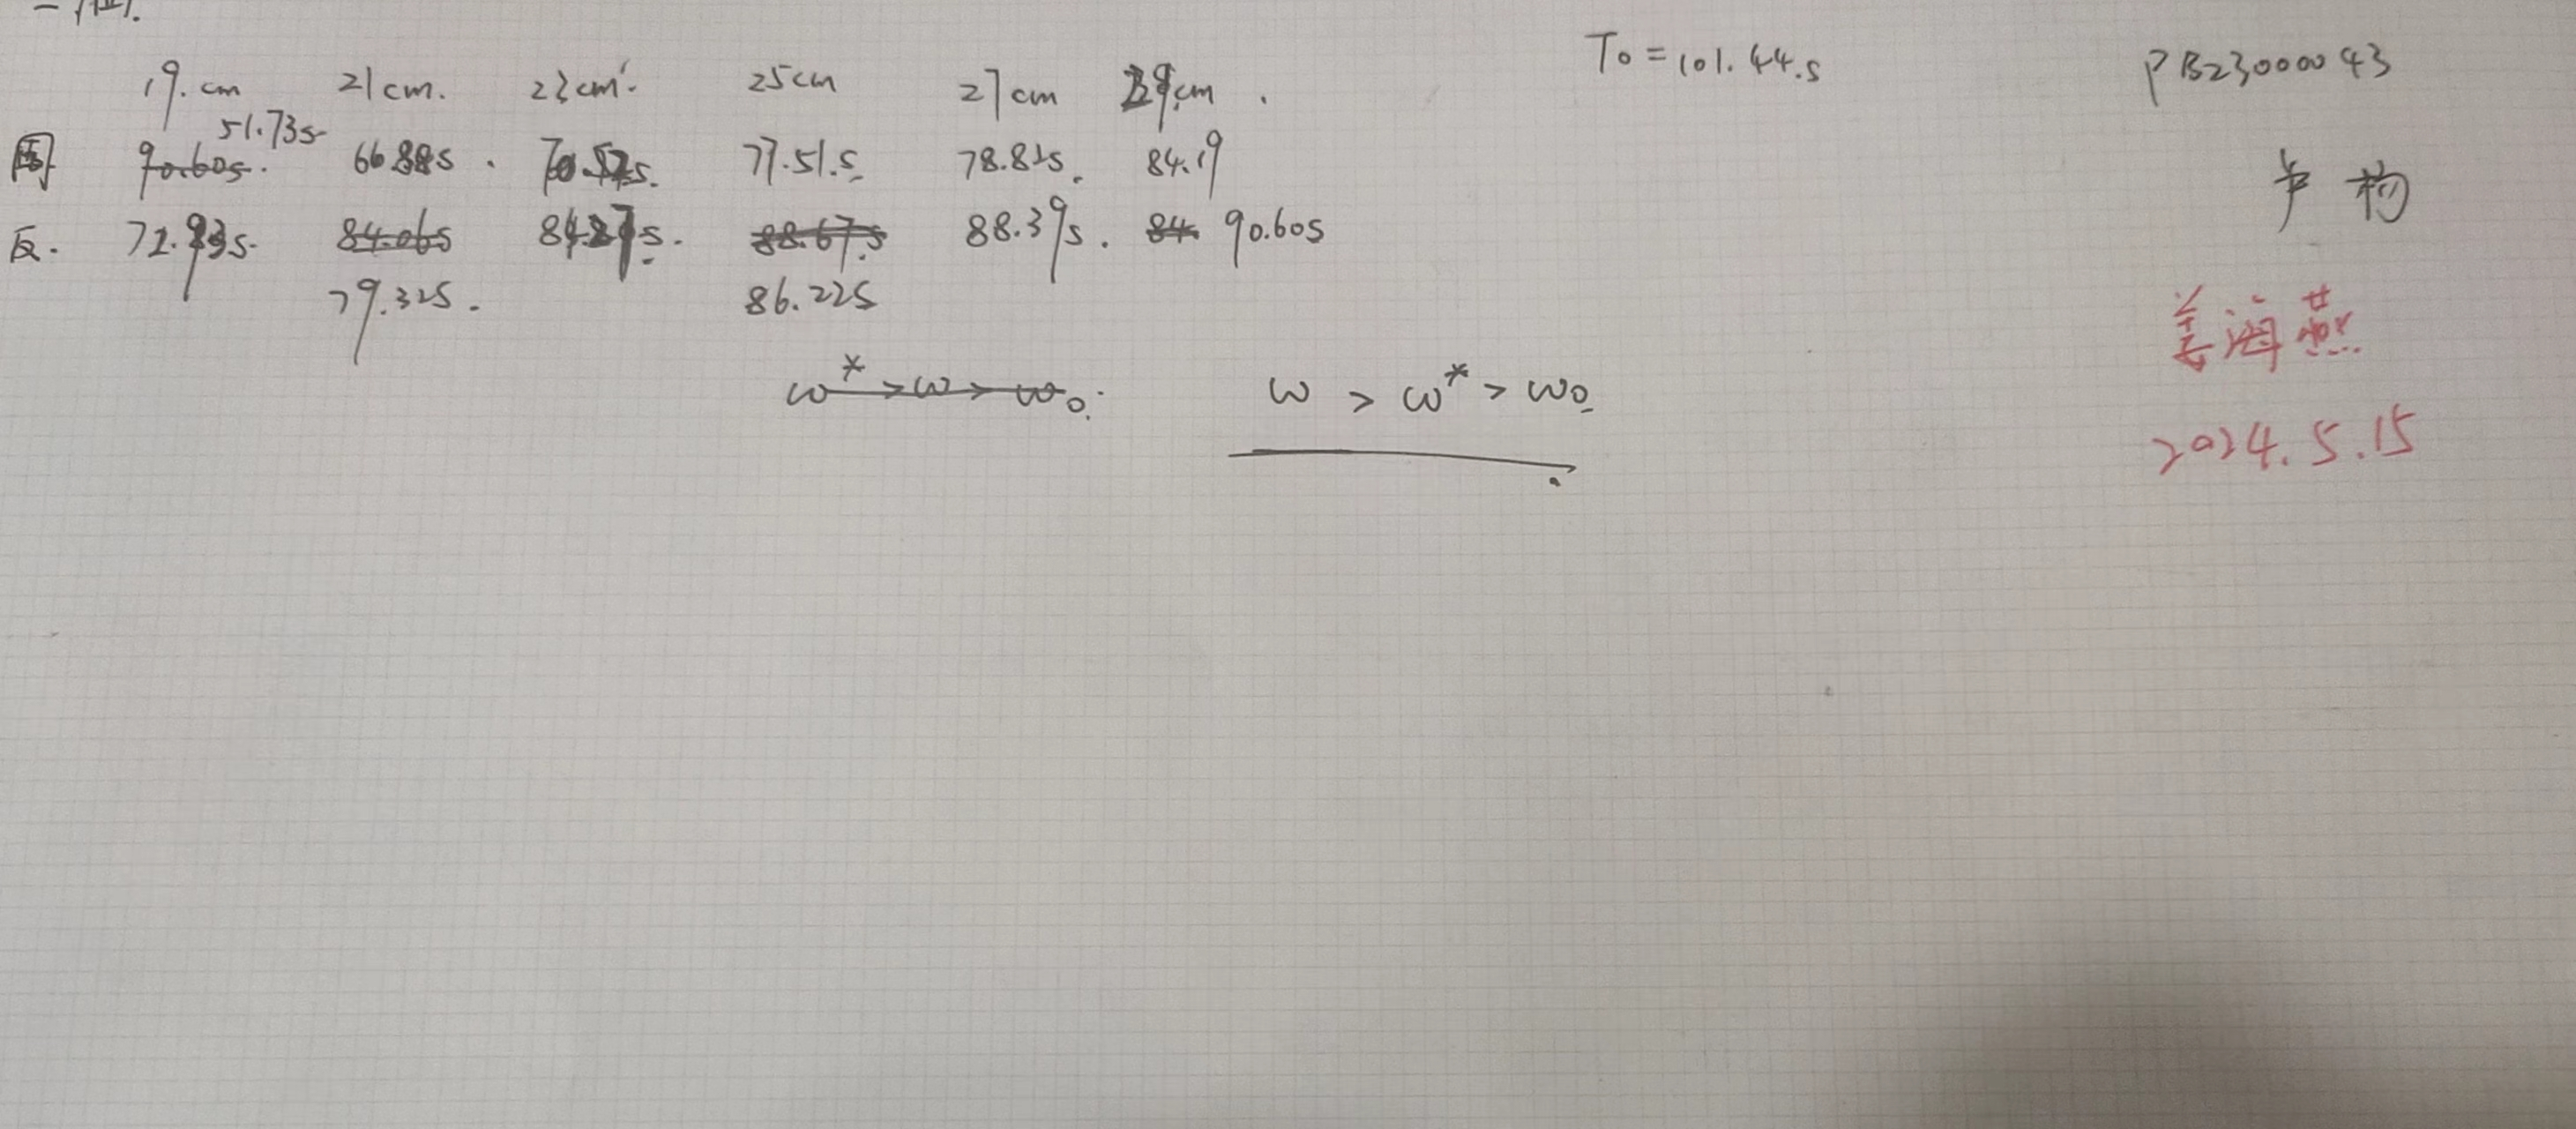
\includegraphics[width=50px]{./img/1.jpg}
% %     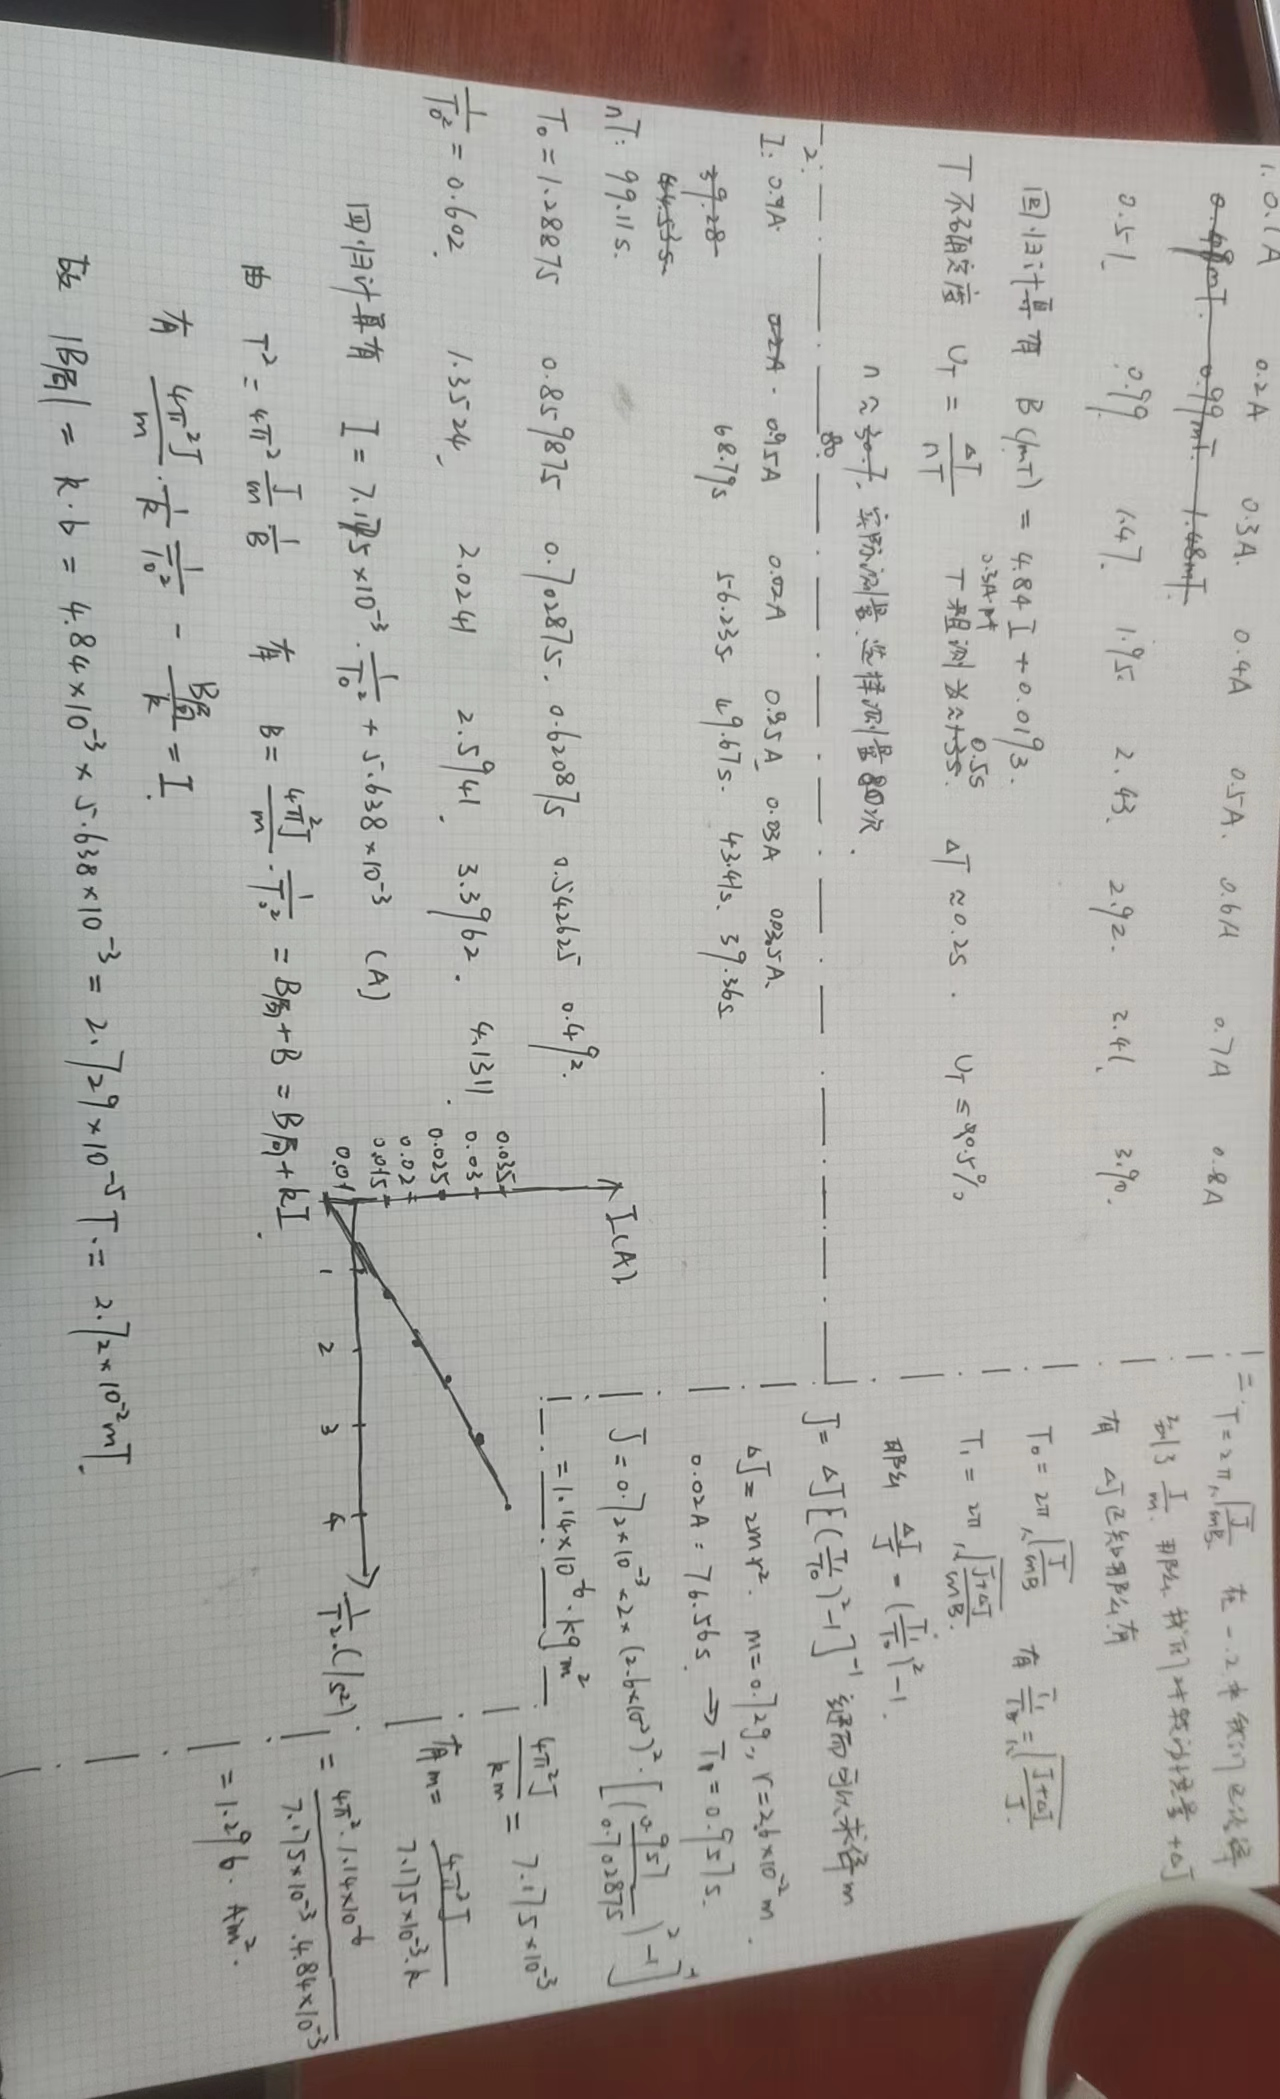
\includegraphics[width=30px,angle=90]{./img/2.jpg}
% % \end{figure}

% \begin{figure}[H]
%     \centering
%     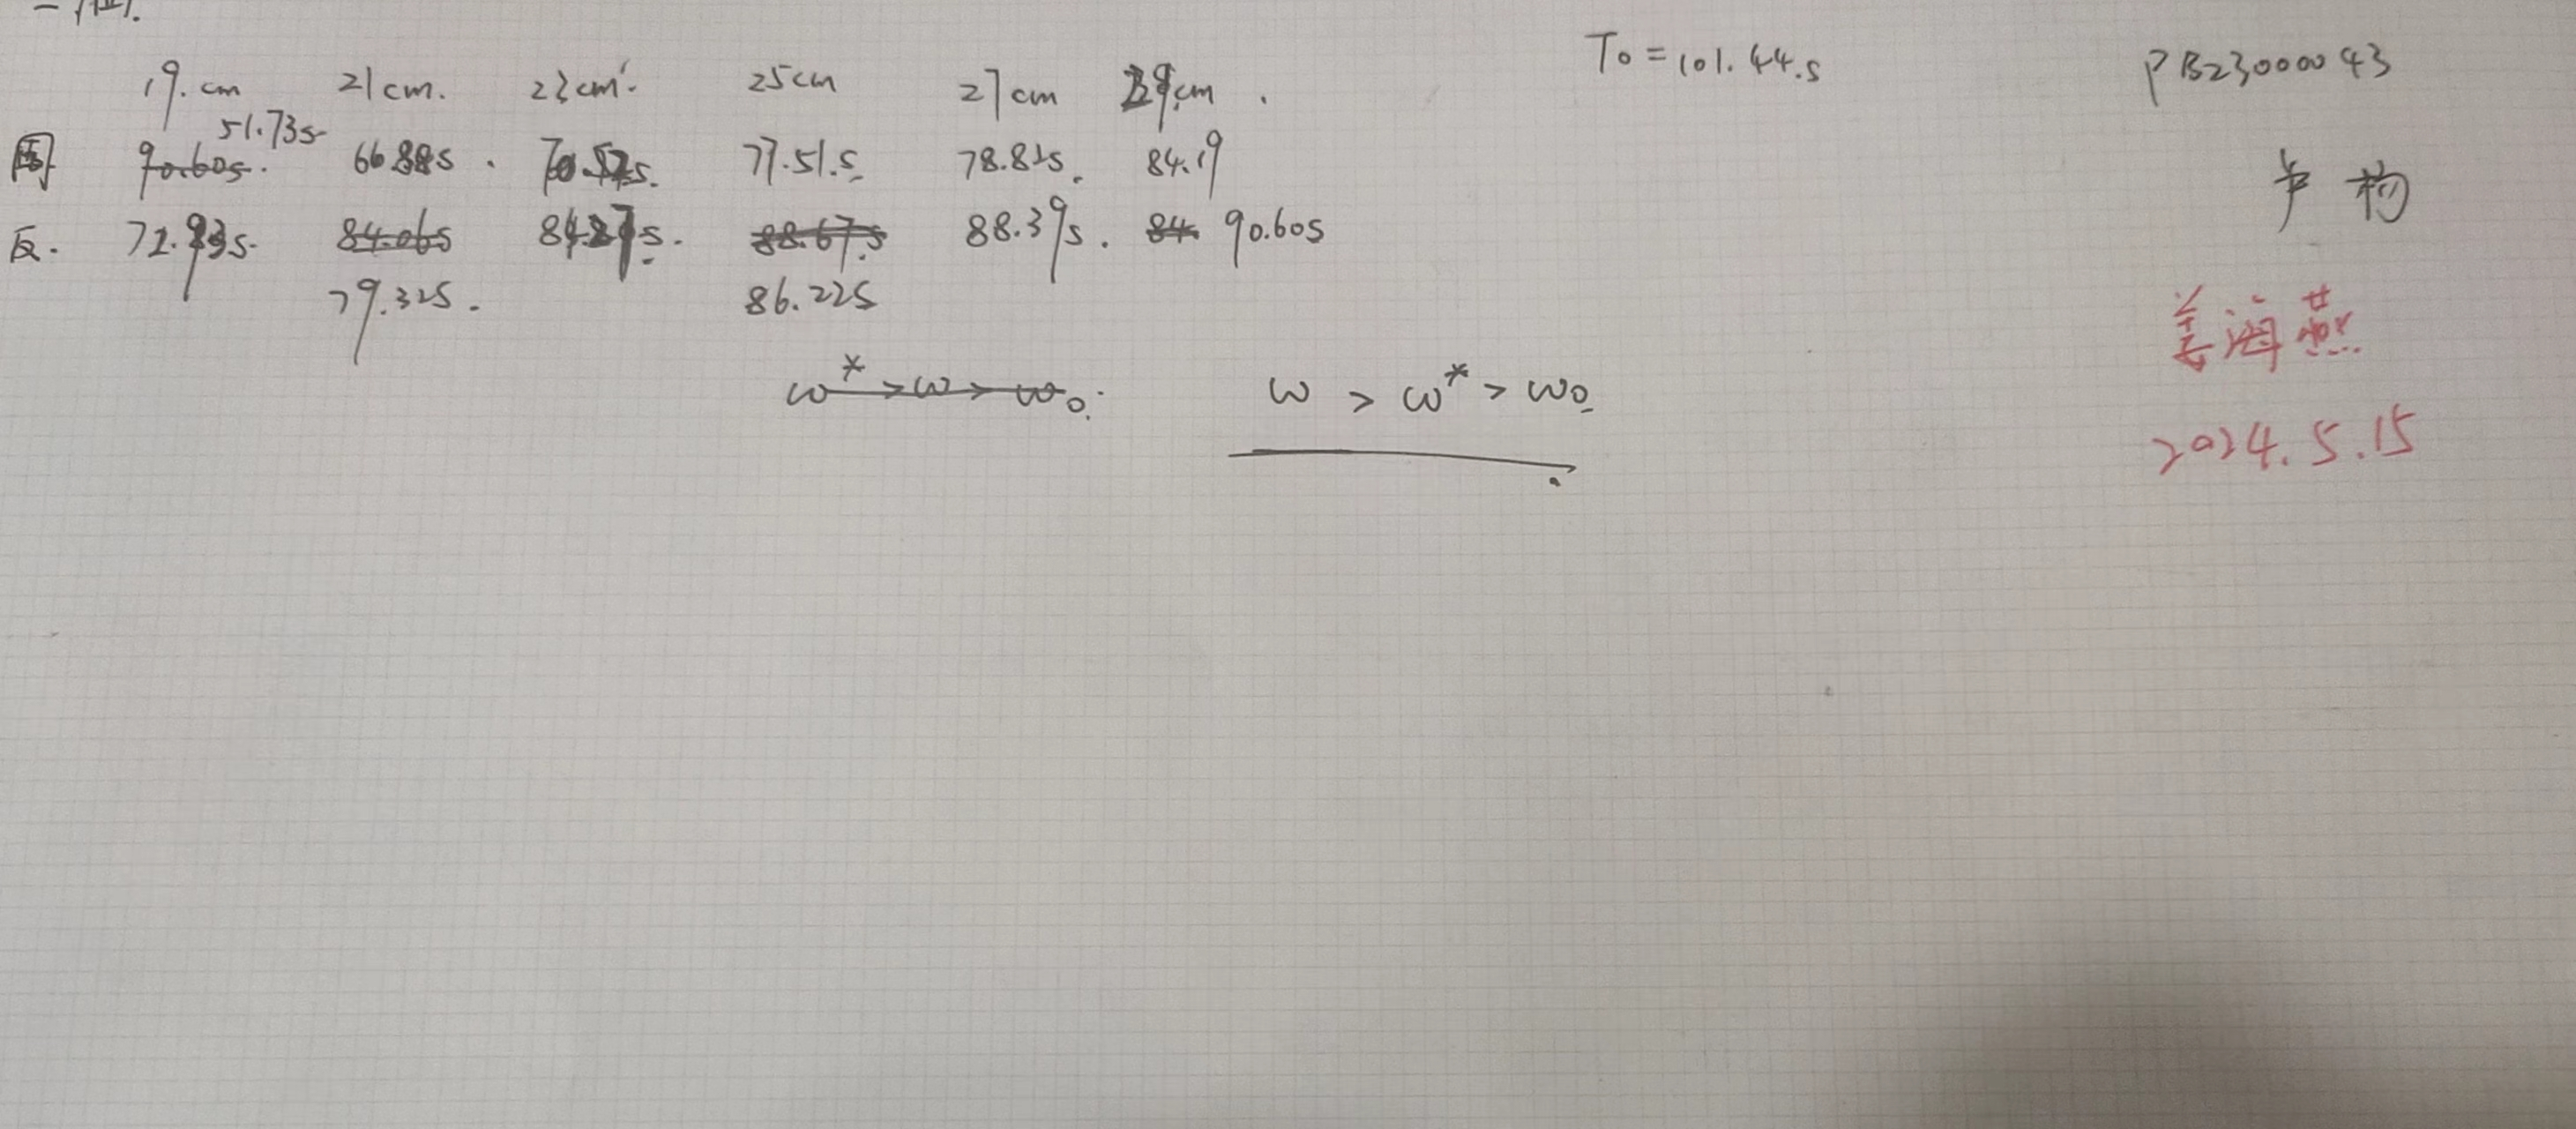
\includegraphics[width=15cm]{./img/1.jpg}
%     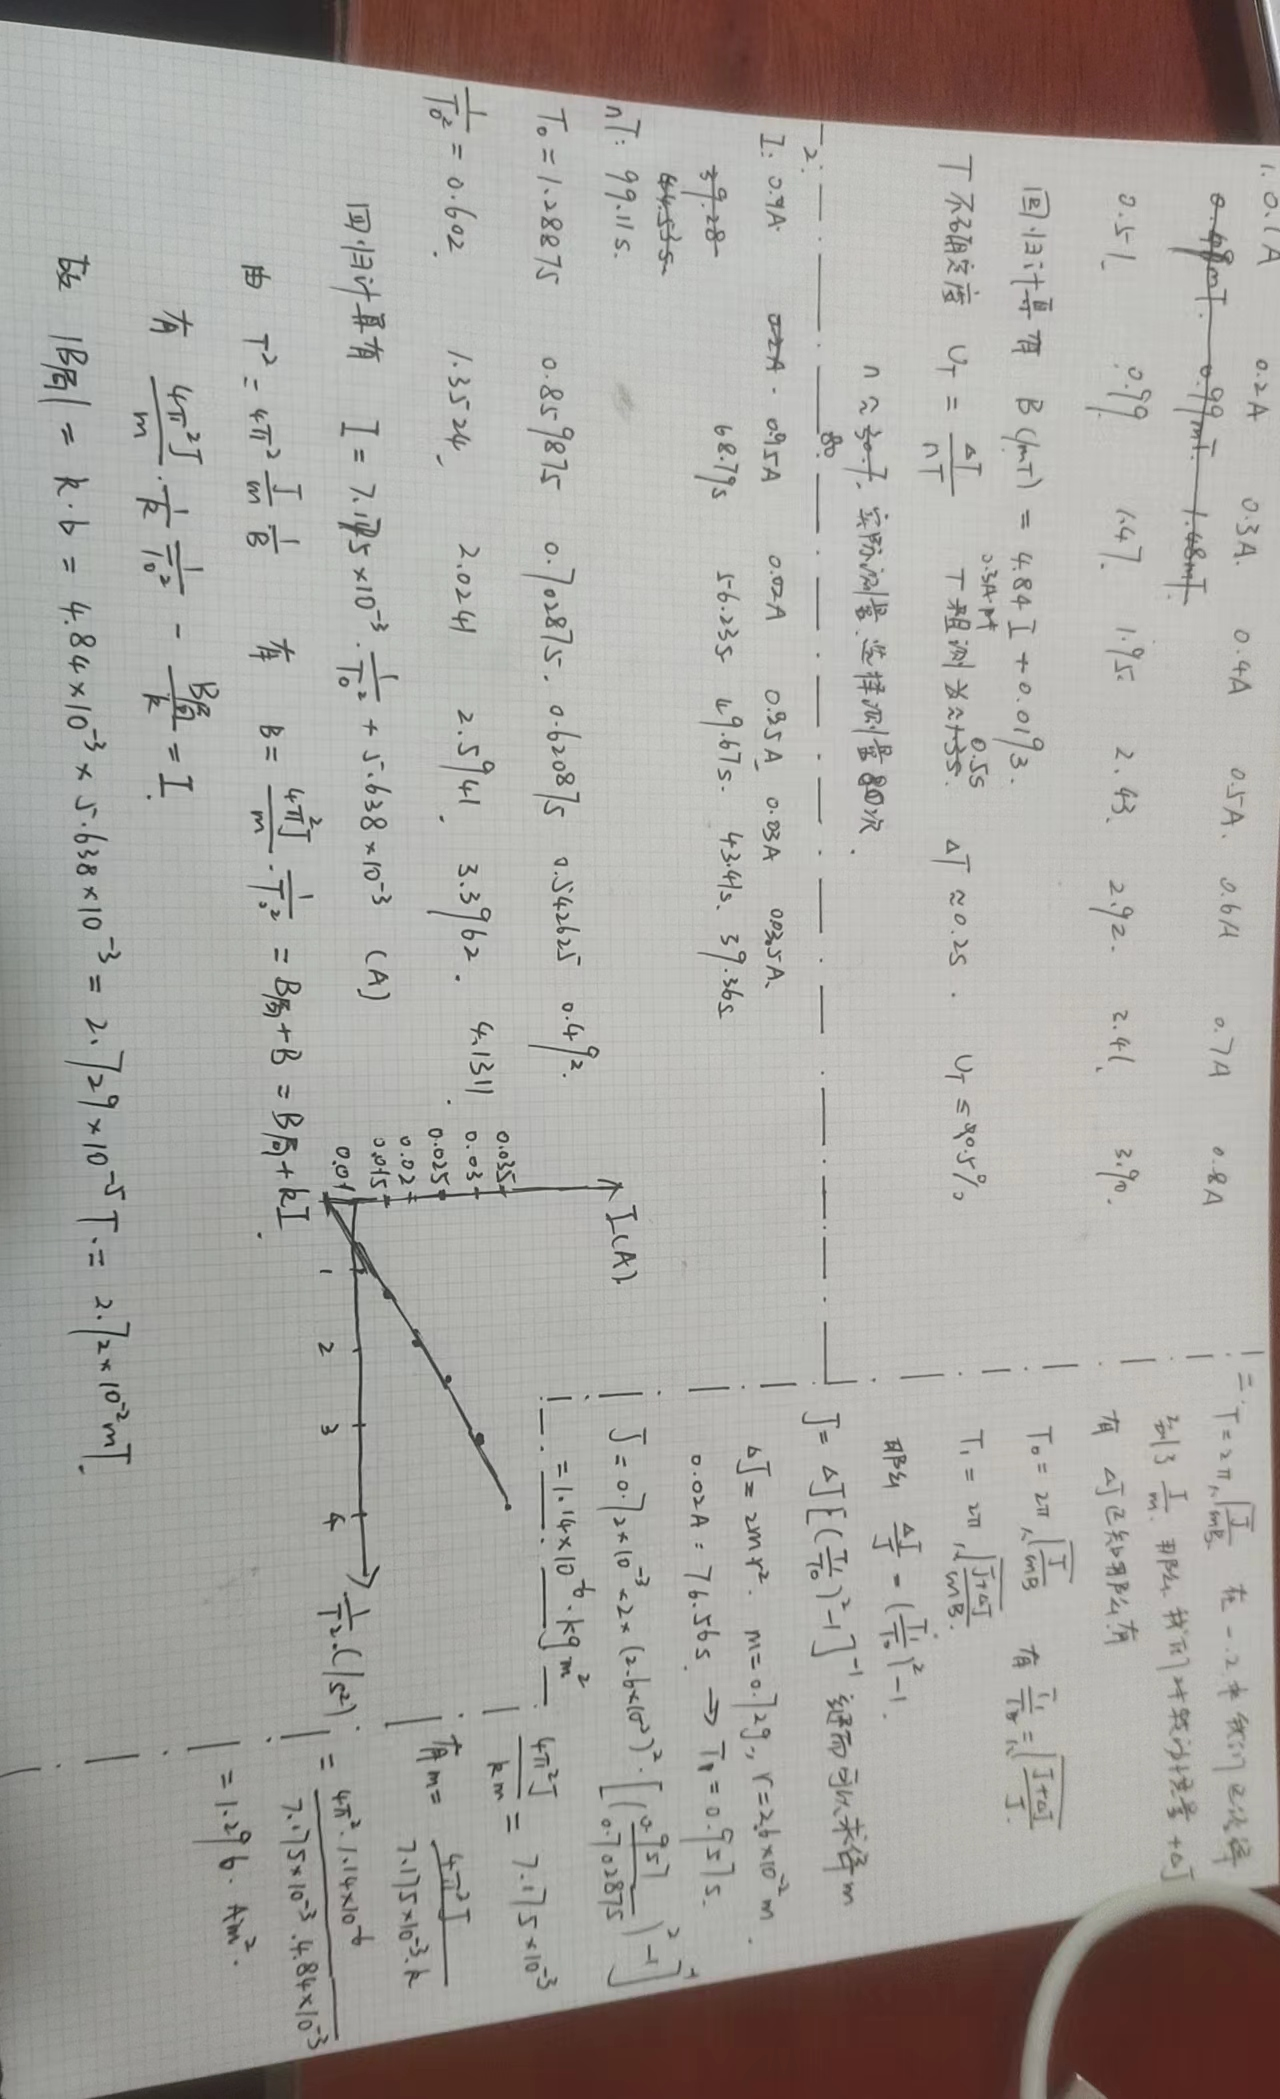
\includegraphics[width=9.2cm,angle=90]{./img/2.jpg}
% \end{figure}

\end{document}